% !TEX encoding = UTF-8
% !TEX TS-program = pdflatex
% !TEX root = ../Tesi.tex

%************************************************

%************************************************
Segue un overview del metodo generale utilizzato, in sezione \ref{section:approcci} e degli approcci specifici, in sezione \ref{section:data_sources}, per ogni Social Media in esame da cui è stato estratto un argumentation framework.

\section{Metodologie di Mining}
\label{section:approcci}
L'estrazione di argomenti prende in esame la struttura che i commenti in uno specifico Social Network possono assumere. In tutte le fonti analizzate un commento può considerarsi una risposta ad un solo altro commento, questo restituisce una struttura ad albero che, partendo dal nodo radice, si dirama attraverso relazioni di risposta. Di seguito viene descritta l'estrazione dell'albero dei commenti in sezione \ref{subsection:albero_commenti} ed un tentativo di estrazione di un grafo considerando come nodi gli utenti in sezione \ref{subsection:grafo_utenti}.

\subsection{Albero dei commenti}
\label{subsection:albero_commenti}
Per la costruzione dell'albero dei commenti serve costruire un grafo orientato della conversazione $\mathcal{G = ⟨V, E⟩}$, dove i nodi $v \in \mathcal{V}$ sono commenti ed esiste un arco $(v_1,v_2) \in \mathcal{E}$ se il commento $v_1$ risponde al commento $v_2$.

La struttura dell'albero può variare in base alla sorgente dei dati in esame, ad esempio alcuni Social Network pongono un limite al numero di livelli dell'albero, principalmente per motivi di presentazione.
Estrarre delle semantiche da Argumentation Framework ricavati dall'albero della conversazione equivale ad estrarre i commenti che soddisfano i requisiti delle varie semantiche.

\subsection{Grafo degli utenti}
\label{subsection:grafo_utenti}
Invece di considerare i commenti come argomenti, può essere considerato argomento ogni utente nella conversazione, e creare archi nel Argumentation Framework risultante tra due utenti se un utente ha risposto almeno una volta ad un altro utente. Più formalmente costruire un grafo orientato $\mathcal{G = ⟨V, E⟩}$, dove i nodi $v \in \mathcal{V}$ sono utenti ed esiste un arco $(v_1,v_2) \in \mathcal{E}$ se l'utente $v_1$ ha risposto almeno una volta all'utente $v_2$.

In questo modo se ogni commento nell'albero della conversazione ha un utente univoco, l'Argumentation Framework risultante sarà comunque un albero, mentre se un utente risponde ad almeno due (o più) utenti il suo nodo nell'$AF$ avrà due (o più) archi uscenti, e se più commenti dello stesso utente vengono risposti da due (o più) utenti, il suo nodo nell'$AF$ avrà due (o più) archi entranti.
Estrarre delle semantiche da Argumentation Framework ricavati dal grafo degli utenti equivale ad estrarre gli utenti che soddisfano i requisiti delle varie semantiche.

\subsection{Pesi delle relazioni}
\label{subsection:weight}
Le relazioni di risposta nell'albero dei commenti vengono pesate in base alla combinazione di similarità e sentiment dei commenti della relazione.

\subsubsection{Similarity}
La \textit{similarity} è ricavata attraverso l'embedding dei testi dei commenti ricavati da un modello di Word2Vec pre-addestrato sulle news di Google \cite{googlenewsmodel}. Gli Word Embedding sono un insieme di tecniche per la rappresentazione vettoriale delle parole di un vocabolario, introdotti per la prima volta in \cite{mikolov2013distributed}, i quali sono capaci di catturare il contesto delle parole all'interno di un documento attraverso la \textit{distributional semantics}. I vettori risultanti codificano proprietà linguistiche nello spazio vettoriale e nella distanza tra di essi, ad esempio è possibile fare analogie come mostrato in figura \ref{fig:analogy}.

\begin{figure}
    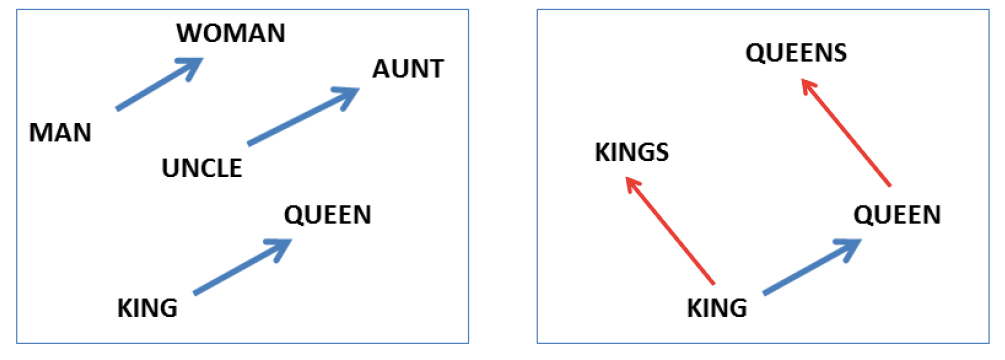
\includegraphics[width=\linewidth]{Immagini/king-queen.png}
    \caption{Analogie tra vettori.}
    \label{fig:analogy}
\end{figure}

L'emebedding dei testi dei commenti è ottenuto facendo la media degli embedding delle parole contenute. Infine la similarità tra due testi $c_1$ e $c_2$ si ricava con:

$$cosineSimilarity(c_1, c_2) = \frac{c_1 \cdot c_2}{||c_1|| ||c_2||}$$

che restituirà quindi un risultato compreso $\in [0, 1]$.

\subsubsection{Sentiment}
La \textit{sentiment analysis} si riferisce all'utilizzo dell'elaborazione del linguaggio naturale per identificare, estrarre e quantificare sistematicamente informazioni soggettive. L'analisi del sentiment è ampiamente applicata per analizzare social media per una varietà di applicazioni. Il valore è ricavato attraverso VADER \cite{hutto2014vader} uno strumento di analisi del sentimento basato su regole che è ideato specificamente per individuare la polarità nei testi espressi nei social media, ad esempio:

    $$sentiment(\ "\textbf{:)}" \ ) = 0.4588$$
    $$sentiment(\ "\textbf{:(}" \ ) = -0.4404$$

che restituirà quindi un risultato compreso $\in [-1, 1]$.

\subsubsection{Peso finale}
Il peso finale dell'arco è ottenuto prendendo in considerazione la similarità tra i commenti, in modo da pesare di più commenti che parlano dello stesso argomento e di meno commenti che parlano di argomenti diversi, ed il sentiment in modo da capire se i commenti sono in accordo o in disaccordo attraverso:

$$weight = similarity_{c_1 c_2} \cdot sentiment_{c_1} \cdot sentiment_{c_2}$$

che restituirà quindi un risultato compreso $\in [-1, 1]$.

\section{Analisi dei Social Media}
\label{section:data_sources}

\subsection {Twitter} %%%%%%%%%%%%%%%%%%%%%%%%%%%%%%%%%%%%%%%%%%%

Lo scraping del sito Web è vietata dal Twitter Terms of Service, quindi l'unico modo rimane l'accesso tramite API. Per accedere alla piattaforma delle API di twitter è necessario creare un Twitter developer account ed in seguito creare dal portale una applicazione nella quale si dichiara lo scopo dello dell'accesso ai contenuti e si richiedono i relativi permessi. Una volta ottenuta l'approvazione, vengono rilasciati delle credenziali per l'autenticazione agli endpoint, ovvero:

\begin{itemize}
    \item consumer key
    \item consumer secret
    \item access token
    \item access token secret
\end{itemize}

I contenuti messi a disposizione sono i Tweet pubblici, cercando parole chiave specifiche attraverso le Search API o chiedendo esempi di Tweet a determinati account attraverso le User API. Inoltre è possibile richiedere tweet specifici conoscendone l'id.

\subsubsection{Overview}
Al momento non è disponibile l'accesso alle conversazioni, la richiesta di tweet tramite le Search API o le User API restituisce solo un sottoinsieme dei tweet ed inoltre c'è un limite al numero di richieste giornaliere. Questo rende difficile cercare di ricostruire le conversazioni dai tweet restituiti dalla query. 

\subsubsection{Ricostruire la conversazione}
\label{ricostruire-conv}
La richiesta ad un determinato topic restituisce un campione di massimo 1000 tweet recenti.
Fra gli attributi presenti nei tweet è presente il campo \textbf{"in reply to status id"} che, se presente, contiene l'id del tweet al quale il tweet corrente sta rispondendo. Questo id può essere utilizzato per cercare di ricostruire la conversazione, facendo una richiesta tramite API per avere il tweet risposto e, se questo a sua volta risponde ad un altro tweet, continuare a seguire la catena di risposte (la conversazione). Per qualsiasi tweet con questo campo, possiamo:
\begin{itemize}
    \item trovare il tweet a cui quello corrente sta rispondendo, quindi ripetere la procedura per ogni tweet con questo attributo avvalorato in modo da ottenere delle sequenze di tweet.
    \item Una volta create le sequenze di tweet, se queste contengono elementi in comune, unire le sequenze creando un grafo della conversazione.
    \item Valutare la bontà della conversazione ottenuta mediante euristiche come il numero di elementi (tweet) nel grafo, la presenza di diramazioni o il numero di utenti distinti.
\end{itemize}

Quindi costruire grafo orientato della conversazione $\mathcal{G = ⟨V, E⟩}$, dove i nodi $v \in \mathcal{V}$ sono tweet ed esiste un arco $(v_1,v_2) \in \mathcal{E}$ se l'attributo \textbf{"in reply to status id"} di $v_1$ contiene l'id di $v_2$.

Tuttavia le API forniscono l'accesso solo ad un campione dei tweet, quindi potrebbe non essere possibile recuperare dei tweet quando si tenta di ricostruire la conversazione. Un'altra limitazione proviene dal numero di tweet iniziale che è possibile ottenere in risposta alla query, che risulta essere massimo 1000, dei quali è necessario filtrare i tweet che contengono il campo \textbf{"in reply to status id"} avvalorato, numero che può variare di molto (di solito circa il 10\%). Inoltre le conversazioni risultano quasi sempre essere sequenze lineari di nodi, ovvero grafi con archi in entrata $\leq 1$ ed archi in uscita $\leq 1$ come rappresentato in figura \ref{fig:comment-twitter} ed il grafo ricostruito cambia in base al momento della richiesta.

\begin{figure}[ht]
    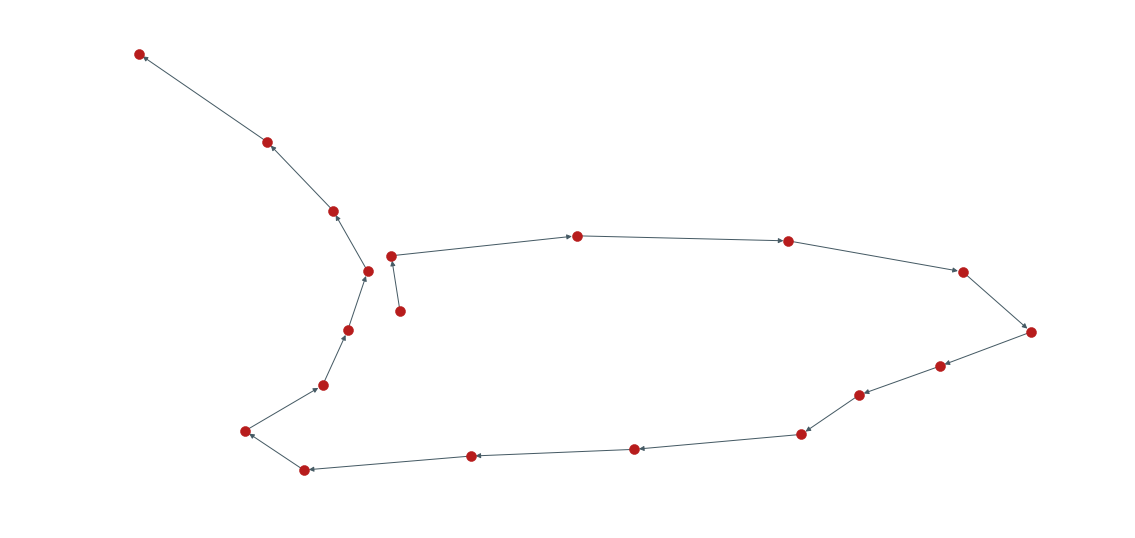
\includegraphics[width=\linewidth]{Immagini/twitter.png}
    \caption{Rappresentazione del grafo della conversazione, utilizzando come nodi i commenti.}
    \label{fig:comment-twitter}
\end{figure}

\subsubsection {Utenti come nodi}
Un altro approccio utilizzato, indipendente dalle funzionalità messe a disposizione da Twitter o dalle Twitter API, consiste nel considerare gli utenti in una conversazione come nodi e creare un arco orientato tra due utenti se esiste almeno un tweet di risposta tra i due, più formalmente: costruire un grafo orientato $\mathcal{G = ⟨V, E⟩}$, dove i nodi $v \in \mathcal{V}$ sono utenti ed esiste un arco $(v_1,v_2) \in \mathcal{E}$ se esiste almeno un tweet con utente $v_1$ e con l'attributo \textbf{"in reply to status id"} contenente l'id di un tweet appartenente all'utente $v_2$.

Anche qui si ripropongono i problemi presentati nella sezione precedente \ref{ricostruire-conv}, tuttavia il grafo risultante presenta nodi con archi in entrata $\geq 1$ ed archi in uscita $\geq 1$, come rappresentato in figura \ref{fig:users-twitter}.

\begin{figure}[ht]
    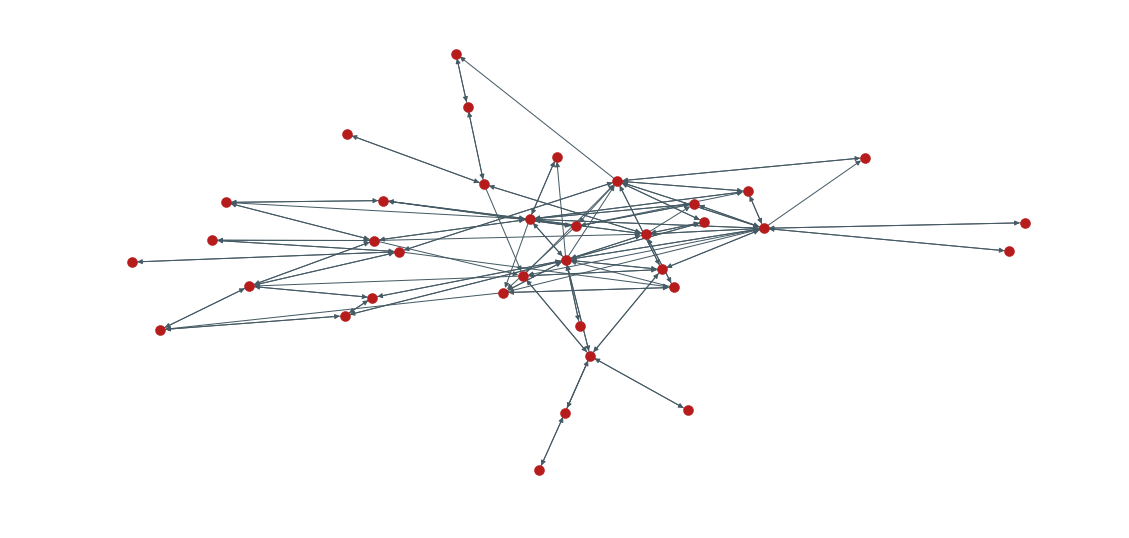
\includegraphics[width=\linewidth]{Immagini/twitter-users.png}
    \caption{Rappresentazione del grafo della conversazione, utilizzando come nodi gli utenti.}
    \label{fig:users-twitter}
\end{figure}



%%%%%%%%%%%%%%%%%%%%%%%%%%%%%%%%%%%%%%%%%%%%%%%%%%%%%%%%%%%%%%%
%%%%%%%%%%%%%%%%%%%%%%%%%%%%%%%%%%%%%%%%%%%%%%%%%%%%%%%%%%%%%%%
%%%%%%%%%%%%%%%%%%%%%%%%%%%%%%%%%%%%%%%%%%%%%%%%%%%%%%%%%%%%%%%
%%%%%%%%%%%%%%%%%%%%%%%%%%%%%%%%%%%%%%%%%%%%%%%%%%%%%%%%%%%%%%%
%%%%%%%%%%%%%%%%%%%%%%%%%%%%%%%%%%%%%%%%%%%%%%%%%%%%%%%%%%%%%%%


\subsection {Stackoverflow} %%%%%%%%%%%%%%%%%%%%%%%%%%%%%%%%%%%%%%%%%%%

\begin{itemize}
    \item create account at https://stackapps.com/
    \item register an app
    \item b
\end{itemize}

\subsubsection {Overview}
\subsubsection {API}

\subsubsection {Commenti}
\subsubsection {Utenti}


%%%%%%%%%%%%%%%%%%%%%%%%%%%%%%%%%%%%%%%%%%%%%%%%%%%%%%%%%%%%%%%
%%%%%%%%%%%%%%%%%%%%%%%%%%%%%%%%%%%%%%%%%%%%%%%%%%%%%%%%%%%%%%%
%%%%%%%%%%%%%%%%%%%%%%%%%%%%%%%%%%%%%%%%%%%%%%%%%%%%%%%%%%%%%%%
%%%%%%%%%%%%%%%%%%%%%%%%%%%%%%%%%%%%%%%%%%%%%%%%%%%%%%%%%%%%%%%
%%%%%%%%%%%%%%%%%%%%%%%%%%%%%%%%%%%%%%%%%%%%%%%%%%%%%%%%%%%%%%%

\subsection {Reddit} %%%%%%%%%%%%%%%%%%%%%%%%%%%%%%%%%%%%%%%%%%%

\begin{itemize}
    \item create account at 
    \item register an app
    \item b
\end{itemize}


\subsubsection {Overview}
\subsubsection {API}

\subsubsection {Commenti}
\subsubsection {Utenti}

% Fatti generati argument/1, attac- k/2, support/2, rel_weight/3

% descrizione vader e altri componenti utilizzati

